\documentclass{project}
\usepackage {comment}

\usepackage[colorinlistoftodos]{todonotes}
\usepackage[pdfauthor={Group 14},pdftitle={Software Engineering Group Project, Design Specification},pdftex]{hyperref}
\usepackage{graphicx}

\begin{document}

\title{Software Engineering Group Project}
\subtitle{Design Specification}
\author{Group 14}     
\shorttitle{Design Specification}
\version{1.0}
\status{Released}
\date{2013-12-05}
\configref{SE-14-DESIGN}

\maketitle

\tableofcontents

\newpage

\section{INTRODUCTION}
\subsection{Purpose of this Document}
The purpose of this document is to describe the design of the Walking Tour
Creator and the Walking Tour Displayer applications. It should be read in the
context of the Group Project, taking into account the details of the group
project assignment and the group project quality assurance (QA) plan.
\cite{se.qa.05a} 


\subsection{Scope}
The design specification gives a detailed explanation of how the individual
components of the Walking Tour Creator and the Walking Tour Displayer
applications should be implemented.

This document should be read by the Android application development team and
the website development team.


\subsection{Objectives}

The main objective of this document are:

\begin{itemize}
\item To describe the main components of the Walking Tour Creator and the
Walking Tour Displayer
\item To show the dependancies between the components and the communication
between the application and web server
\item To provide interface details for each of the main classes in the Walking
Tour Creator
\end{itemize}

\newpage

\section{DECOMPOSITION DESCRIPTION}
\subsection{Programs in system}
The system is composed of two programs:
\begin{itemize}
\item The Walking Tour Creator Android application
\item The Walking Tour Displayer website
\end{itemize}


\subsubsection{Walking Tour Creator}
The Walking Tour Creator is an application to allow the user can create walks
on a mobile device for them to be uploaded to the server. It implements the
requirements (FR1), (FR2), (FR3), (FR4), (FR5), (FR6), (FR7), (FR9), (PR1) and
must conform with the requirements (EIR1), (PR2), (DC1), (DC2).\cite{se.qa.rs}

This application will use a GUI as a means for the user to create a walk. The
user will be able to walk around an area and the GPS component of their device
will capture the route that they take. Along the route, they can mark points of
interest, which contains a description and optionally a photo. Once the user
has completed the walk, they can choose to either discard their creation or
upload it to the Walking Tour Displayer.

\subsubsection{Walking Tour Displayer}
The Walking Tour Displayer is website for viewing walks created by users via
the Walking Tour Creator. It implements the requirements (FR8), (FR9), (PR1)
and must conform to the requirements (EIR1), (PR2), (DC1), (DC2),
(DC3).\cite{se.qa.rs}

The walks are stored in a MySQL database with the attributes specified in
(DC3). The database will be queried by the website and allow the user to select
a walk. The selected walk would then be displayed on a map, and the user can
select a points of interest along the route of the walk.

\newpage

\subsection{Significant classes in each program}
\subsubsection{Significant classes in Walking Tour Creator}
\emph{MainAppActivity}. This is the main class of the application.

\emph{WalkCreatorActivity}. This is an activity panel holding the UI for
recording the walk. It also has a Location Listener running in the backgorund recording the users walk

\emph{Walk}. This contains a list of the coordinates of the route that the user
is creating, and the metadata of the walk.

\emph{PointOfInterest}. This contains a point of interest in the route, which
is a coordinate with a description and optionally a photo of what is in that.

\subsubsection{Significant functions in Walking Tour Displayer}
\emph{intialize}. This JavaScript function creates an embedded Google Map on
the page.

\emph{addMarker}. This JavaScript function takes coordinates as parameters and
sets a marker on the map using them.

\emph{addPath}. This JavaScript function takes two coordinates as parameters
and it sets a path on the map using them.


\subsection{Mapping requirements onto classes}
\begin{tabular}{|l |l |}
\hline
\emph{Requirement} & \emph{Classes providing requirement} \\
\hline
FR1 & MainAppActivity \\
\hline
FR2 & WalkCreatorActivity, Walk \\
\hline
FR3 & WalkCreatorActivity, Walk, PointOfInterest  \\
\hline
FR4 & WalkCreatorActivity \\
\hline
FR5 & WalkCreatorActivity \\
\hline
FR6 & WalkCreatorActivity \\
\hline
FR7 & MainAppActivity \\
\hline
FR8 & N/A \\
\hline
FR9 & WalkCreatorActivity \\
\hline
\end{tabular}


\newpage


\section{DEPENDENCY DESCRIPTION}
\subsection{Component Diagrams}

\subsubsection{Component Diagram for Walking Tour Creator}
\begin{figure}[h] 

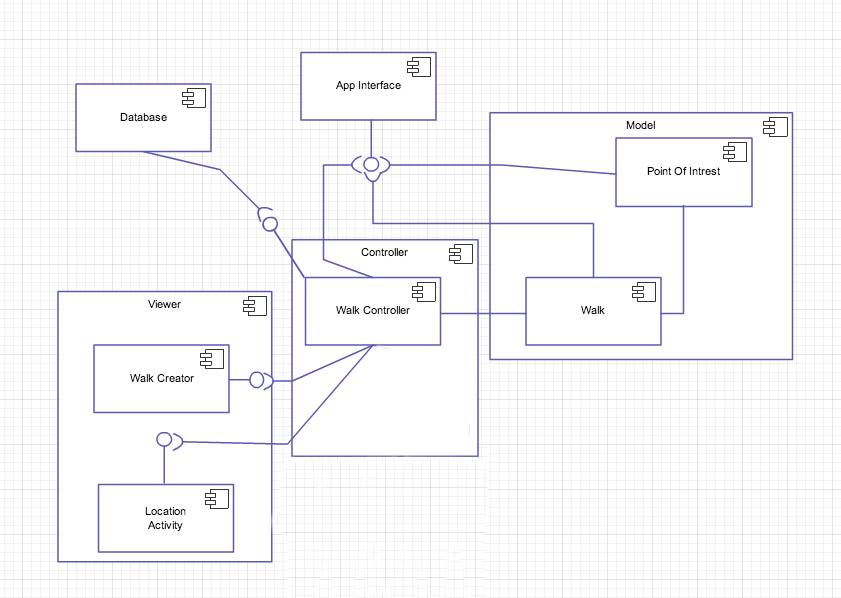
\includegraphics[width=15cm]{NewComponentDiagram.jpg}
\end{figure}

\newpage

\subsubsection{Component Diagram for Walking Tour Displayer}
\begin{figure}[h] 
    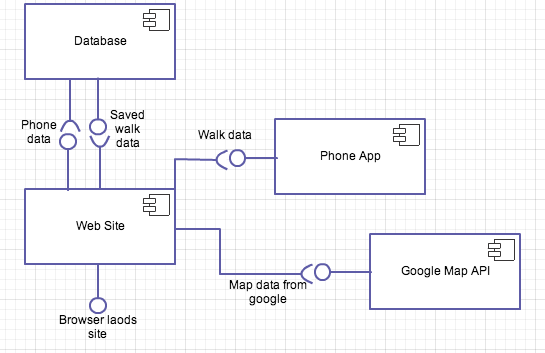
\includegraphics[width=15cm]{compontent_diagram_WTD.png}
\end{figure}

\newpage

\subsection{Inheritance Relationships}
The class with the most dependency is the WalkController, which has GPS
recording, walk creator and location activity. Just about all of the classes
need WalkController and this is where the app will send the data from the walk
made from the app to the website. Walk has a dependency with PointOfInterest
because it calls the gets and sets from that class. WalkCreatorActivity does GPS recording passes to controller then to walk. WalkCreatorActivity has the most dependancies.

For basic understanding of the dependencies of the Walking Tour Creator:
\begin{itemize}
\item Walk controller on walk creator and Location activity.
\item Walk on point of interest and walk controller.
\item Web site on walk controller.
\end{itemize}

The website has dependancies on the database to be able to get data of the
walks and to be able display them on the map and also show the description of
the walk on the side panel next to the map. Finally, the phone has a dependency
on the website because the data from the walk needs to go though the website to
be able to send the data to the database.      

For basic understanding of the dependencies of the Walking Tour Creator:
\begin{itemize}
\item Website on database and Google Maps API.
\item Phone app on website. 
\end{itemize}

\newpage

\section{INTERFACE DESCRIPTION}
\subsection{MainAppActivity interface specification}
\begin{verbatim}/**
 * This activity is shown when the user opens the app.
 * It has a single button which allows the user to "Create a walk". 
 * This button launches the "WalkDetailsActivity" Activity.
 *
 * @author Group 14
 */
public class WalkDetailsActivity {
   /**
    * This is the method which launches the "WalkCreatorActivity" Activity.
    * This is called when the user presses the "Create route" button.
    */
   public void createWalk();
}\end{verbatim}

\subsection{WalkDetailsActivity interface specification}
\begin{verbatim}/**
<<<<<<< HEAD
 * This interface is used represent a point of interest.
 * This will store a String name, String description,
 * Location object, and optional String representing
 * a picture associated with the point
 * @author Group14
 *
 */
public interface IPointOfInterest extends Parcelable {
   
   /**
    * This method is used to set the IPointOfInterest's name
    * @param name String representing the new name of the IPointOfInterest
    */
   public void setName(String name);
   
   /**
    * This method is used to get the IPointOfInterest's name
    * @return String representing the name of the IPointOfInterest
    */
   public String getName();
   
   /**
    * This method is used to set the IPointOfInterest's description
    * @param desc String representing the new description of the IPointOfInterest
    */
   void setDescription(String desc);
   
   /**
    * This method is used to get the IPointOfInterest's description
    * @return String representing the IPointOfInterest's description
    */
   public String getDescription();
   
   /**
    * This method is used to set the picture of the IPointOfInterest.
    * This must be a valid path to a picture in the filesystem.
    * @param picture String representing the location of the picture in the filesystem
    */
   public void addPicture(String picture);
   
   /**
    * This method is used to get the picture of the IPointOfInterest
    * @return A string representing the location on the filesystem of the picture
    */
   public String getPicture();
   
   /**
    * This method is used to get the IPointOfInterest's latitude
    * @return A double representing the IPointOfInterest's latitude
    */
   public double getLatitude();
   
   /**
    * This method is used to get the IPointOfInterest's longitude
    * @return A double representing the IPointOfInterest's longitude
    */
   public double getLongitude();
   
   /**
    * This method is used to get the IPointOfInterest's timestamp.
    * @return long timestamp in the unix epoch format.
    */
   public long getTime();
   
   /**
    * This method is used to get the IPointOfInterest's Location object
    * @return A Location object, representing the GPS location of the IPointOfInterest
    */
   public android.location.Location getLocation();
   
}
}\end{verbatim}

\subsection{JsonPackage interface specification}
\begin{verbatim}
package uk.ac.aber.group14.model;

/**
 * This interface is used to convert an IWalk to a JSON String
 * @author Group14
 *
 */
public interface IJsonPackager {
   
   /**
    * This takes an IWalk and converts it into a JSON String
    * @param w The walk which will be converted
    * @return A String containing the walk represented as a JSON object
    */
   public String JSONify(IWalk w);
   
}
\end{verbatim}

\newpage


\subsection{Walk interface specification}
\begin{verbatim}
package uk.ac.aber.group14.model;


/**
 * This interface is used to represent a walk
 * This stores a collection of Location objects,
 * a collection of IPointOfInterest objects,
 * a String name, String short description, and String
 * long description.
 * @author Group14
 *
 */
public interface IWalk extends Parcelable{

   /**
    * This method is used to add a single IPointOfInterest to the IWalk
    * @param point The point to add to the IWalk
=======
 * This activity requires the user to enter a name, short description, and long
 * description of the walk. When they press the "Create route" button this
 * launches the "WalkCreatorActivity" giving it the details to create the walk
 * from.
 *
 * @author Group 14
 */
public class WalkDetailsActivity {
}\end{verbatim}

\newpage

\subsection{WalkController interface specification}
\begin{verbatim}/**
 * This interface is used to control the IWalk object. 
 * When instantiated, this will create an IWalk and an AGPSLocationLogger.
 * It allows the viewer to add a point of interest, finish, or cancel the walk.
 *
 * @author Group 14
 */
public interface IWalkController {
   /**
    * This method takes an IPointOfInterest as an argument and adds it to the
    * IWalk.
    */
   public void addPointOfInterest(IPointOfInterest poi);
    
   /**
    * This method will stop the AGPSLocationLogger, remove the current IWalk,
    * and return to the MainAppActivity.
    */
   public void cancelWalk();
   
  
}\end{verbatim}

\newpage

\subsection{Walk interface specification}
\begin{verbatim}/**
 * This interface is what actually stores the data of the walk. 
 * This contains a list of Location objects for the walk, a list of
 * IPointOfInterest objects, a name, a short description, and a long
 * description
 *
 * @author Group 14
 */
public interface IWalk {
   /**
    * This method takes an IPointOfInterest object and adds it to the list of
    * points of interest.
>>>>>>> doc
    */
   public void addPointOfInterest(IPointOfInterest point);
   
   /**
<<<<<<< HEAD
    * This method is used to add a LinkedList of Location objects to the IWalk
    * @param locations The Locations to add to the IWalk
    */
   public void addLocations(java.util.LinkedList<android.location.Location> locations);
   
   /**
    * This method is used to set the name of the IWalk
    * @param name String representing the name of the walk
    */
   public void setName(String name);
   
   /**
    * This method is used to set the short description of the IWalk
    * @param desc String representing the short description of the IWalk
    */
   public void setShortDescription(String desc);
   
   /**
    * This method is used to set the long description of the IWalk
    * @param desc String representing the long description of the IWalk
    */
   public void setLongDescription(String desc);
   
   /**
    * This method is used to return the points of interest
    * as an array of PointOfInterest
    * @return An array of type PointOfInterest representing all the points of interest in the IWalk
=======
    * This method adds a LinkedList of Location objects to the walk. 
    * This is to allow the controller to put a large number of Location objects
    * into the walk once the walk is finished and the logger as returned all of
    * the points of data.
    */
   public void addLocations(LinkedList locations);
   
   /**
    * This sets the walk's user-viewable name.
    */
   public void setTitle(String name);
   
   /**
    * This sets the walks short (<100 char) description.
    */
   public void setShortDesctiption(String Sdesc);

   /**
    * This sets the walk's long (<1000 char) description. 
    */
   public void setLongDescription(String Ldesc);
   
   /**
    * This returns an array of all of the IPointOfInterest objects. 
    * This is to be used when finishing and uploading the walk.
>>>>>>> doc
    */
   public IPointOfInterest[] getPointsOfInterest();
   
   /**
<<<<<<< HEAD
    * This method is used to return the GPS locations as an array of
    * type Location
    * @return An array of type Location representing all of the Locations in the IWalk
    */
   public android.location.Location[] getLocations();
   
   /**
    * This method is used to get the name of the IWalk
    * @return A String representing the name of the IWalk
    */
   public String getName();
   
   /**
    * This method is used to get the short description of the IWalk
    * @return A String representing the short description of the IWalk
=======
    * This returns an array of all of the walk's Location objects. 
    * This is used when finishing and uploading the walk.
    */
   public android.location.Location[] getLocations();

   /**
    * This returns the String containing the walk's name.
    */
   public String getTitle();
   
   /**
    * This returns the string containing the walk's short (<100 characters)
    * description.
>>>>>>> doc
    */
   public String getShortDescription();
   
   /**
<<<<<<< HEAD
    * This method is used to get the long description of the IWalk
    * @return A String representing the long description of the IWalk
    */
   public String getLongDescription();
   
   /**
    * This method is used to add a single Location to the IWalk
    * @param location The Location to add to the walk
    */
   public void addLocation(Location location);
   
   /**
    * This method is used to get the number of Location objects
    * in the IWalk
    * @return An int representing the number of Location objects in the IWalk
    */
   public int getNumberLocations();
   
   /**
    * This method is used to get the number of IPointOfInterest objects
    * in the IWalk
    * @return An int representing the number of IPointOfInterest objects in the IWalk
    */
   public int getNumberPOI();
=======
    * This returns the string containing the walk's long (<1000 characters)
    * description.
    */
   public String getLongDescription();
   
   
>>>>>>> doc
}

\end{verbatim}

\newpage

\section{DETAILED DESIGN}
\subsection{Sequence diagrams}

\begin{figure}[h] 

   
\includegraphics[width=15cm]{New_Sequence_Diagram_Group_Project_14.png}
    
\end{figure}

\newpage

\subsection{Significant algorithms}
<<<<<<< HEAD
\textbf{SetMarkers}
SetMarkers basically takes points from the database and plots them using the LineBetweenPoints function and the google API. It takes in the latitude and longitude from a 2 dimensional array and plots the points on the map

\textbf{LineBetweenPoints}
LineBetweenPoints uses the Google API to go from of marker to the next and plots a route in between them. See the JSON format specification for the data transmission algorithms.
=======
\subsection{SetMarkers}
SetMarkers basically takes points from the database and plots them using the LineBetweenPoints function and the google API. It takes in the latitude and longitude from a 2 dimensional array and plots the points on the map
/textbf{LineBetweenPoints}
LineBetweenPoints uses the google API to go from of marker to the next and plots a route in between them. Before we discovered the API,we thought to write our own version in java. 
see the JSon document for the data transmission algorithms.
>>>>>>> doc
\begin{comment}
\subsubsection{LocationLoggerService algorithm}
This algorithm is used to decide which GPS locations to keep and which to
discard. This is done in order to remove unnecessary points and conserve
memory on the phone as well as space in the database.

This encompasses several algorithms. First it decides which method it picks by
looking at averages over several points and looking at the standard deviation
to see if any anomalies might indicate a change in direction. This is separated
into several different algorithms:

\textbf{Straight line} \\
No change of direction across several points (likely 4 or more, but this could
be changed in the algorithms implementation as a variable) will cause the
points in the middle to be removed. This will look at the standard deviation of
points and general direction of points to ensure it's not slowly going round a
corner.

\textbf{Corner} \\
It will be possible to test for corners above 60° easily by testing for a
straight line followed by another straight line in a completely different
direction. This will probably rely on the previous algorithm to thin out some
points before this can take effect.

\textbf{Slight turn} \\
Detecting a slight turn with a low angle of difference will be difficult. It
will be quite similar to detecting a corner but will likely require more points
of data to detect that the change of direction is not just an anomaly in a
straight line. We can make a vector out of the direction of each 3 points in
succession with a direction and detect when several lines in one direction are
suddenly followed by several lines in a slightly different direction.

\textbf{Rounded turn} \\
Detecting a rounded turn will be the most challenging algorithm. This will be
used for large, sweeping corners and will most likely require either a large
loop or some recursion. Due to the constant change of direction across the turn
this will not be picked up by any of the other algorithms. This itself will
ignore the corner and leave the points in place, allowing the corner's GPS
points to be preserved.
\end{comment}

\subsection{Significant data structures}
The data structures we will be using are the IPointOfInterest interface and the
IWalk interface.

The IWalk interface will be implemented by a class and will hold all of the
points of interest. It is the current plan to use a LinkedList due to it being
dynamic in size. If the team member implementing the interface has a compelling
enough reason to use an alternative means of storing them then they can do. Due
to it being an interface this will be up to whoever implements it - the public
methods will remain the same.

The IPointOfInterest will be used to store the data about a point of interest.
For storing the pictures it is again likely that a LinkedList will be used.

The Location objects will be stored in a LinkedList in the walk
whilst they are being recorded. This will allow us to quickly and easily add
new Location objects to the end of it. Unlike an array, we will not need to
repeatedly recreate the list with a larger amount of memory each time a new
location is added.

\clearpage
\addcontentsline{toc}{section}{REFERENCES}
\begin{thebibliography}{5}
\bibitem{se.qa.rs} \emph{Software Engineering Group Projects}
Requirements Specification. \\
C. J. Price and B.P.Tiddeman, SE.QA.RS. 1.4 Release.
\bibitem{se.qa.05a} \emph{Software Engineering Group Projects}
Design Specification Standards. \\
C. J. Price, N.W.Hardy, B.P.Tiddeman, SE.QA.05a. 1.7 Release.
\end{thebibliography}
\addcontentsline{toc}{section}{DOCUMENT HISTORY}
\section*{DOCUMENT HISTORY}
\begin{tabular}{|l | l | l | l | l |}
\hline
Version & CCF No. & Date & Changes made to Document & Changed by \\
\hline
0.1 & N/A & 2013-12-04 & Initial creation & tht5, jam66, meo9 \\
\hline
0.2 & N/A & 2013-12-04 & Moved document to project template & jmt14 \\
\hline
1.0 & N/A & 2013-12-04 & Added remaining content & jmt14, tht5, jam66 \\
\hline
<<<<<<< HEAD
1.1 & N/A & 2014-1-29 & Updating and making changes to content & meo9, jam66 \\
\hline
1.2 & N/A & 2014-2-13 & Updating interface specifications and formatting. & meo9 \\
=======
1.1 & N/A & 2013-1-29 & Updating and making changes to content & meo9, jam66 \\
>>>>>>> doc
\hline
\end{tabular}
\label{thelastpage}

\end{document}